\documentclass{article}

\usepackage[utf8]{inputenc} % allow utf-8 input
\usepackage[T1]{fontenc}    % use 8-bit T1 fonts
\usepackage[colorlinks=true, linkcolor=black, citecolor=blue, urlcolor=blue]{hyperref}       % hyperlinks
\usepackage{url}            % simple URL typesetting
\usepackage{booktabs}       % professional-quality tables
\usepackage{amsfonts}       % blackboard math symbols
\usepackage{amsmath,amssymb}% more math symbols
\usepackage{chngcntr}		% more math symbols
\usepackage{dsfont}			% font with double lines for sets
\usepackage{microtype}      % micro typography
\usepackage{graphicx}		% including images
\graphicspath{ {./figs/} }
\usepackage{setspace}		% spacing
\usepackage[german]{babel}	% german quotation marks etc.
\usepackage{pdfpages}		% to include entire pdf pages in appendix etc.
\usepackage{marvosym}		% more math symbols
\usepackage{mathtools}		% more math symbols
\usepackage{enumitem}		% better custom enumerations
\setlist[enumerate, 1]{label=\roman*)}
\usepackage{mathrsfs}
\usepackage{tikz-cd}		% drawing custom diagrams
\usepackage[a4paper]{geometry} % a4 paper
\usepackage{enumitem,setspace,graphicx}
\DeclareGraphicsExtensions{.pdf,.png,.eps,.jpg}


\def\then{\ensuremath{\Rightarrow}} % =>;
\def\since{\ensuremath{\Leftarrow}}
\def\iff{\ensuremath{\Leftrightarrow}} % genau dann wenn
\def\to{\ensuremath{\rightarrow}} % ->;
\def\Oh{\ensuremath{\mathcal{O}}} % Landau-Notation beispielsweise $\Oh(n)$
\def\N{\ensuremath{\mathbb{N}}}
\def\R{\ensuremath{\mathbb{R}}}
\def\C{\ensuremath{\mathbb{C}}}
\def\S{\ensuremath{\mathbb{S}}}
\def\id{\ensuremath{\text{id}}}
\newcommand{\angles}[1]{\left\langle #1 \right\rangle}

\newcommand{\includetask}[2][pages=-]{
	\includepdf[#1]{#2}
	\addtocounter{subsection}{1}
}

%pretty epsilon
\let\oldepsilon\epsilon
\let\epsilon\varepsilon
\let\varepsilon\oldepsilon
%pretty phi
\let\oldphi\phi
\let\phi\varphi
\let\varphi\oldphi

% ---

% --- DIESES 3 FELDER SIND AUSZUFÜLLEN ---
\def\sheetNumber{01}
\def\names{Linus Mußmächer} 
\def\sumPoints{30} 

\setcounter{section}{\sheetNumber}

\begin{document}

\begin{doublespace}
	\begin{center}
		\textbf{\Large{Übungsblatt \sheetNumber}}\\
		\textbf{\Large{Stochastik 2}}\\
		Abgabe von: \textbf{\names}\\
		\today
	\end{center}
	%	\hfill  {\large Punkte: $\boxed{\qquad  /\; \sumPoints}$}\\
\end{doublespace}

%\vspace{3cm}

%\begin{center}
%	
\includegraphics[width=0.5\textwidth]{pi.png}
%\end{center}

%\newpage

\subsection{Zentralübung}

\begin{enumerate}[label=(\alph*)]
	\item Wir zeigen zuerst, dass es sich um eine Verteilungsfunktion handelt, indem wir die Bedingungen aus 3.34 überprüfen.
	      \begin{enumerate}
		      \item \textbf{Stetigkeit}: Für $t > 1$ und $t < 1$ ist die Funktion sicherlich stetig, und wegen $1 - 1^{-\alpha}=0$ ist sie auch am Übergangspunkt $t = 1$ stetig. Somit ist $F_\alpha$ nach dem Klebelemma stetig und damit insbesondere rechtsseitig stetig.
		      \item \textbf{Monotonie}: Für $t < 1$ ist $F_\alpha|_{t < 1} \equiv 0$, also monoton wachsend. Für $t \geq 1$ ist wegen $\alpha > 0$ die Funktion $t^{-\alpha}$ (streng) monoton fallend, also $1 - t^{-\alpha}$ (streng) monoton wachsend und außerdem stets positiv. Somit ist $F_\alpha$ insgesamt monoton wachsend.
		      \item \textbf{Grenzverhalten}: Es ist
		            \begin{equation*}
			            \lim_{n \to -\infty} F_\alpha(n) \overset{n < 1}{=} \lim_{n \to -\infty} 0 = 0 \qquad \lim_{n \to \infty} F_\alpha(n) \overset{n > 1}{=} \lim_{n \to \infty} 1 - \underbrace{n^{-\alpha}}_{\to 0} = 1 - 0 = 1
		            \end{equation*}
	      \end{enumerate}
	      Somit ist $F_\alpha$ eine Verteilungsfunktion. Wir berechnen das Integral $\int_{-\infty}^{t} f_\alpha(t) dt$. Für $t < 1$ folgt
	      \begin{equation*}
		      \int_{-\infty}^{t} f_\alpha(\tau) d\tau = \int_{-\infty}^{t} 0 d\tau = 0 = F_\alpha(t)
	      \end{equation*}
	      und für $t > 1$ erhalten wir
	      \begin{align*}
		      \int_{-\infty}^{t} f_\alpha(\tau) d\tau = \int_{-\infty}^{1} 0 d\tau + \int_{1}^{t} \frac{\alpha}{\tau^{\alpha + 1}} d\tau = \alpha \left[\frac{1}{-\alpha} \tau^{-\alpha}\right]_1^t = - \frac{1}{\alpha} t^{-\alpha} - \left( - \frac{\alpha}{\alpha} \right) = F_\alpha(t)
	      \end{align*}
	      und somit ist $f_\alpha$ die Dichte von $F_\alpha$.
	\item Es gilt für $\alpha \neq n$:
	      \begin{align*}
		      \mathds{E}[X^n] & = \int_{-\infty}^{\infty} x^n dF_\alpha(x) = \int_{-\infty}^{\infty} x^n f_\alpha(x) dx                                                                                    \\
		                      & = \int_{1}^{\infty} x^n \cdot \alpha x^{-\alpha - 1} dx = \lim_{t \to \infty} \int_{1}^{t} \alpha x^{n - \alpha - 1} dx                                                    \\
		                      & = \lim_{t \to \infty} \alpha \left[\frac{1}{n - \alpha} x^{n - \alpha}\right]_1^t = \lim_{t \to \infty} \frac{\alpha}{n - \alpha} \left(t^{n-\alpha} - 1^{n-\alpha}\right) \\
	      \end{align*}
	      Für $\alpha > n$ gilt nun $\lim_{t \to \infty} t^{n - \alpha} = 0$ und damit $\mathds{E}[X^n] = \frac{\alpha}{n - \alpha} (0 - 1) = \frac{\alpha}{\alpha - n}$. Für $\alpha < n$ wiederum ist $\lim_{t \to \infty} t^{n - \alpha} = \infty$ und damit auch $\mathds{E}[X^n] = \infty$. \\
	      Wir betrachten noch den Fall $\alpha = n$:
	      \begin{equation*}
		      \mathds{E}[X^n] = \lim_{t \to \infty} \int_{1}^{t} \alpha x^{n - \alpha - 1} dx = \lim_{t \to \infty} \int_{1}^t \alpha x^{-1} dx = \alpha \int_{1}^t \left[\ln(x)\right]_1^t = \lim_{t \to \infty} \ln(t)  - \ln(1) = \infty
	      \end{equation*}
	      Somit ist die geforderte Gleichheit gezeigt. Sei nun $\alpha > 2$. Dann existieren das 1. und 2. Moment, und wir können die Varianz berechnen:
	      \begin{equation*}
		      \mathds{V}[X] = \mathds{E}[X^2] - \mathds{E}[X]^2 = \frac{\alpha}{\alpha - 2} - \left(\frac{\alpha}{\alpha - 1}\right)^2 = \frac{\alpha^2(\alpha-2) - \alpha (\alpha-1)^2}{(\alpha - 2)(\alpha - 1)^2} = \frac{\alpha}{(\alpha - 2)(\alpha - 1)^2}
	      \end{equation*}
	\item Sei zuerst $t < 0$. Dann ist
	      \begin{equation*}
		      F_Y(t) = \mathds{P}(Y \leq t) = \mathds{P}(\alpha \ln(X) \leq t) = \mathds{P}(X \leq \underbrace{\exp(t/\alpha)}_{<1}) = 0\text{,}
	      \end{equation*}
	      also durch Ableiten auch $f_Y(t) = 0$ für alle $t<0$. Sei nun $t \geq 0$. Dann gilt analog
	      \begin{align*}
		      F_Y(t) & = \mathds{P}(Y \leq t) = \mathds{P}(\alpha \ln(X) \leq t) = \mathds{P}(X \leq \exp(t/\alpha))    \\
		             & = F_\alpha(\underbrace{\exp(t/\alpha)}_{\geq 1}) = (1 - \exp(t/\alpha)^{-\alpha}) = 1 - \exp(-t)
	      \end{align*}
	      und Ableiten liefert
	      \begin{equation*}
		      f_Y(t) = \exp(-t)
	      \end{equation*}
	      Somit folgt insgesamt $f_Y(t) = \exp(-t) \cdot \mathds{1}_{[0, \infty)}$, also $Y \sim \mathrm{Exp}(1)$.
\end{enumerate}

\subsection{}

\begin{enumerate}[label=(\alph*)]
	\item Wir verwenden Beispiel 3.54, da die Dichte der Normalverteilung stetig ist. Dann gilt
	      \begin{equation*}
		      f_{Y}(t) = \frac{f_X(\sqrt{t}) + f_X(\sqrt{-t})}{2 \sqrt{t}} \cdot \mathds{1}_{[0, \infty)}
	      \end{equation*}
	      Weiterhin ist
	      \begin{align*}
		      f_X(\sqrt{x}) = \frac{1}{\sqrt{2 \pi}} \exp\left(- \frac{1}{2}\sqrt{x}^2\right) = \frac{1}{\sqrt{2 \pi}} \exp\left(- \frac{1}{2} |x|\right) \\
		      f_X(-\sqrt{x}) = \frac{1}{\sqrt{2 \pi}} \exp\left(- \frac{1}{2}(-\sqrt{x})^2\right) = \frac{1}{\sqrt{2 \pi}} \exp\left(- \frac{1}{2} |x|\right)
	      \end{align*}
	      wobei wir die Betragsstriche aufgrund von $t \geq 0$ auch weglassen können. Somit folgt
	      \begin{equation*}
		      f_{Y}(y) = \frac{\exp\left(- y / 2\right)}{\sqrt{2 \pi y}} \cdot \mathds{1}_{[0, \infty)}
	      \end{equation*}
	\item Da die Dichte der Normalverteilung absolutstetig und $\exp: \R \to \R^+$ stetig differenzierbar mit strikt positiver Ableitung ist, können wir Satz 3.52. anwenden. Dann hat $Z$ die Dichte
	      \begin{align*}
		      f_Z(z) & = \frac{f_U(\exp^{-1}(z))}{|\exp'(\exp^{-1}(z))|} \cdot \mathds{1}_{(0, \infty)} = \frac{\frac{1}{\sigma \sqrt{2 \pi}} \exp\left(-\frac{1}{2} \left(\frac{\ln(z) - \mu}{\sigma}\right)^2\right)}{|z|} \cdot \mathds{1}_{(0, \infty)} \\
		             & = \frac{1}{ \sqrt{2 \pi \sigma^2} z} \exp\left( -\frac{(\ln(z) - \mu)^2}{2\sigma^2}\right)\cdot \mathds{1}_{(0, \infty)}
	      \end{align*}
	\item Es ist
	      \begin{align*}
		      \mathds{E}[Z] & = \int_{-\infty}^{\infty} \exp(x) f_U(x) dx = \int_{-\infty}^{\infty} \frac{1}{\sigma \sqrt{2 \pi}} \exp(x) \exp\left(- \frac{1}{2} \frac{(x - \mu)^2}{\sigma^2}\right) dx
	      \end{align*}
	      Substitution von $x$ durch $\sigma x + \mu$ liefert
	      \begin{align*}
		      \mathds{E}[Z] & = \int_{-\infty}^{\infty} \frac{1}{\sqrt{2 \pi}} \exp(\sigma x + \mu) \exp(-x^2/2) dx = \exp(\mu) \int_{-\infty}^{\infty} \frac{1}{\sqrt{2\pi}} \exp\left(-\frac{1}{2} (x^2 - 2 \sigma x )\right)dx
	      \end{align*}
	      Quadratische Ergänzung:
	      \begin{align*}
		      \mathds{E}[Z] & = \exp(\mu) \int_{-\infty}^{\infty} \frac{1}{\sqrt{2\pi}} \exp\left(-\frac{1}{2} (x^2 - 2 \sigma x + \sigma^2 ) + \frac{1}{2} \sigma^2\right)dx \\
		                    & = \exp(\mu + \sigma^2/2)  \int_{-\infty}^{\infty} \frac{1}{\sqrt{2\pi}} \exp\left(-\frac{1}{2} (x - \sigma)^2\right)dx
	      \end{align*}
	      Der Integrand entspricht nun der Dichte einer Normalverteilung $\mathcal{N}(\sigma, 1)$, wodurch das Integral den Wert $1$ haben muss. Dies zeigt $\mathds{E}[Z] = \exp(\mu + \sigma^2/2)$.

	      Analog betrachten wir
	      \begin{align*}
		      \mathds{E}[Z^2] & = \int_{-\infty}^{\infty} (\exp(x))^2 f_U(x) dx = \int_{-\infty}^{\infty} \frac{1}{\sigma \sqrt{2 \pi}} \exp(2x) \exp\left(- \frac{1}{2} \frac{(x - \mu)^2}{\sigma^2}\right) dx \\
		                      & = \int_{-\infty}^{\infty} \frac{1}{\sqrt{2 \pi}} \exp(2 \sigma x + 2 \mu) \exp\left(- \frac{1}{2} x^2\right) dx                                                                 \\
		                      & = \exp(2 \mu) \int_{-\infty}^{\infty} \frac{1}{\sqrt{2 \pi}}\exp\left(- \frac{1}{2} (x^2 - 4 \sigma x + (2 \sigma)^2) + 4 \sigma^2 / 2\right) dx                                \\
		                      & = \exp(2 \mu + 2 \sigma^2) \int_{-\infty}^{\infty} \frac{1}{\sqrt{2 \pi}}\exp\left(- \frac{1}{2} (x-2\sigma)^2\right) dx
	      \end{align*}
	      Wieder ist der Integrand die Dichte einer Normalverteilung $\mathcal{N}(2 \sigma, 1)$ und das Integral hat den Wert $1$. Es folgt $\mathds{E}[Z^2] = \exp(2 \mu + 2 \sigma^2)$.
\end{enumerate}

\subsection{}

\begin{enumerate}[label=(\alph*)]
	\item Sei $f$ die Wahrscheinlichkeitsverteilung von $X$. Dann gilt:
	      \begin{align*}
		      \mathds{P}[X \geq t] & = \int_{t}^{\infty} f(x) dx \leq \int_{t}^{\infty} \underbrace{\exp(\overbrace{s(x-t)}^{\geq 0})}_{\geq 1} f(x) dx                                    \\
		                           & \leq \int_{t}^{\infty} \exp(s(x-t)) f(x) dx + \underbrace{\int_{-\infty}^{t} \overbrace{\exp(s(x-t))}^{\geq 0} \overbrace{f(x)}^{\geq 0} dx}_{\geq 0} \\
		                           & = \exp(-st) \int_{-\infty}^{\infty} \exp(sx) f(x) dx = \exp(-st) \mathds{E}[\exp(sX)]
	      \end{align*}
	      Dies zeigt die Aussage.
	\item Aus $X \sim \mathcal{N}(0,1)$ folgt $sX \sim \mathcal{N}(0,s^2)$. 1.2 (c) zeigt dann $\mathds{E}[\exp(sX)] = \exp(s^2/2)$.
	\item
\end{enumerate}

\subsection{}

\begin{enumerate}[label=(\alph*)]
	\item Sehr krude Skizze. Dichteverteilung in rot, Graph von $x \mapsto 1 - 1/2 \exp(-2x)$ in blau.
	      \begin{center}
		      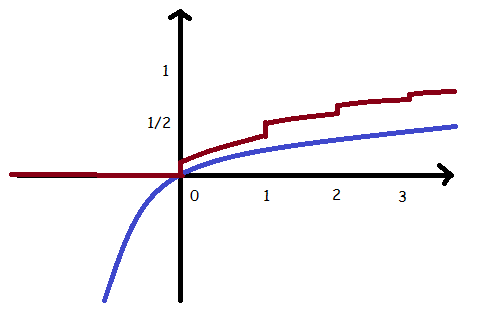
\includegraphics[width=0.4\textwidth]{skizze.png}
	      \end{center}
	\item Wir betrachten
	      \begin{align*}
		      \int_{\R} f d\mu & = \int_{R^-} \underbrace{f}_{=0} d\mu + \int_{\R^+ \setminus \N_0} f d\mu + \int_{\N_0} f d\mu\text{.}
	      \end{align*}
	      Auf $\R \setminus \N_0$ entspricht $\mu$ dem Lebesgue-Maß, da $\delta_k|_{\R\setminus \N_0} \equiv 0$ für alle $k \in \N_0$. Da $\N_0$ bezüglich des Lebesgue-Maßes eine Nullmenge darstellt, können wir also, um das zweite Integral zu erhalten, auch bezüglich des Lebesgue-Maßes von $0$ bis $\infty$ über $\exp(-2x)$ integrieren. Außerdem lässt sich $f$ auf jeder Menge der Form $\{k\}, k \in \N_0$ durch die konstante Funktion $\frac{1}{2e} \frac{1}{k!}$ darstellen. Somit ergibt sich
	      \begin{align*}
		      \int_{\R} f d\mu & = 0 + \int_{0}^{\infty} \exp(-2x) dx + \sum_{k=0}^{\infty} \int_{\{k\}} f d\mu                                                                       \\
		                       & = \left[-\frac{1}{2} \exp(-2x)\right]_0^\infty + \sum_{k=0}^{\infty} \frac{1}{2e} \frac{1}{k!} \underbrace{\mu(\{k\})}_{=1}                          \\
		                       & = -\frac{1}{2} \cdot 0 + \frac{1}{2} \cdot 1 + \frac{1}{2e} \underbrace{\sum_{k = 0}^{\infty} \frac{1^k}{k!}}_{=e^1} = \frac{1}{2} + \frac{1}{2} = 1
	      \end{align*}
	      und damit $\mathds{P}(\R) = 1$.
\end{enumerate}

\end{document}
















